\documentclass[10pt,twocolumn,letterpaper]{article}

\usepackage{cvpr}
\usepackage{times}
\usepackage{epsfig}
\usepackage{graphicx}
\usepackage{amsmath}
\usepackage{amssymb}
\usepackage{booktabs}
\usepackage{floatrow}
\usepackage{epsfig}
\usepackage{epstopdf}
\usepackage{subcaption}
\usepackage{blindtext,graphicx}
\usepackage{multicol}
\usepackage{multirow}
\usepackage{comment}
\usepackage{bm}
\usepackage{float}
\floatstyle{plaintop}
\restylefloat{table}

% Include other packages here, before hyperref.
\graphicspath{{./Images/}}
% If you comment hyperref and then uncomment it, you should delete
% egpaper.aux before re-running latex.  (Or just hit 'q' on the first latex
% run, let it finish, and you should be clear).
\usepackage[breaklinks=true,bookmarks=false]{hyperref}

\cvprfinalcopy % *** Uncomment this line for the final submission

\def\cvprPaperID{2513} % *** Enter the CVPR Paper ID here
\def\httilde{\mbox{\tt\raisebox{-.5ex}{\symbol{126}}}}

% Pages are numbered in submission mode, and unnumbered in camera-ready
%\ifcvprfinal\pagestyle{empty}\fi
\setcounter{page}{1}
\begin{document}

%%%%%%%%% TITLE

\title{Histogram Layer for Texture Classification}


\author{Tyler (Taewook) Kim\\
Kent School\\
1 Macedonia Rd., Kent, CT 06757\\
{\tt\small kimt20@kent-school.edu} 
% For a paper whose authors are all at the same institution,
% omit the following lines up until the closing ``}''.
% Additional authors and addresses can be added with ``\and'',
% just like the second author.
% To save space, use either the email address or home page, not both
\and
Joshua Peeples\\
University of Florida\\
1064 Center Dr, Gainesville, FL 32611\\
{\tt\small jpeeples@ufl.edu}
}

\maketitle
%\thispagestyle{empty}


\begin{abstract}
	 In this paper, we propose a hybrid model that incorporates a stackable, localized histogram layer on convolutional neural network (CNN) for texture analysis applications. Texture classification is a part of texture analysis that focuses on the image’s spatial variation in pixel intensity values and gray levels to classify texture. Instead of using standard histogram operation, we used RBF (Radial Basis Function) to perform a localized binning operation without binning constraints. In order to evaluate the proposed model’s performance, we used six different CNNs comprising of histogram and convolution layer to classify images. Experiments were conducted using the KTH-TIPS 2b dataset and the use of standardization was analyzed during this study. As a result, every network improved performance significantly with standardization, averaging about 6.50\% increase in average overall accuracy. Then, the results were evaluated using confusion matrices, classification metrics, and overall accuracy on the networks standardized data to further evaluate the proposed model. Overall, the proposed model did not necessarily perform better than the standard CNNs, but the histogram CNN performed better on some classes. Future works will include evaluating different initialization methods and parameters such as number of bins, window size, and kernel size.
\end{abstract}

%%%%%%%%% BODY TEXT

%-------------------------------------------------------------------------
\section{Introduction}
 Texture analysis is a process of characterizing texture in an image by spatial variation in pixel intensity values or gray levels. Image texture is a complex visual pattern that is one of the crucial sources of visual information. Some of the texture properties include but not limited to perceived lightness, uniformity, density, roughness, and granulation \cite{Materka98textureanalysis}. This field has been one of the popular research topics in computer vision and machine learning due to its broad impact on numerous fields \cite{Cavalin2017methods}. In medical imaging, texture analysis can quantify the tumor heterogeneity based on MRI, CT, or PET images \cite{Nalepa2014medical}.  In \cite{Pinto2016agri}, researchers implement texture analysis based on leaf images to classify various crop diseases.
\\

 Approaches to texture analysis are generally categorised into four approaches: structural, statistical, model-based, and transform. {\bf Structural analysis} represent texture by microtexture and macrotexture based on pre-defined primitives and the placement rules. {\bf Statistical approaches} represent texture indirectly with methods such as analyzing statistics given by pairs of pixels. {\bf Model-based texture analysis} interprets an image texture using fractal and stochastic models. Lastly, the {\bf transform methods} of texture analysis use methods such as Fourier, Gabor, and Wavelet transforms to interpret texture characteristics such as frequency or size \cite{Materka98textureanalysis}.


%-------------------------------------------------------------------------


\subsection{Related Works}


\par Texture analysis is similar to object recognition but it differs because spatial relationships of patterns in the image are important for most texture analysis approaches, as opposed to points of interests for object recognition \cite{Cavalin2017methods}. Texture-based datasets also have higher dimensionality compared to simple color and shape-based datasets used in object recognition, which makes it a harder task \cite{Basu2018deeptexture}. In order to confront the complexity of texture datasets, several different methods to perform texture analysis have been proposed throughout the literature.
\\


%Traditional Approach
 One of the previous approaches is a traditional approach where researchers used different texture descriptors to observe the region homogeneity and the histograms of these region borders. In \cite{Basu2018deeptexture}, the authors present a review of various hand-crafted features including traditional texture descriptors such as Local Binary Patterns (LBP) \cite{Ojala2002lbp} and Gray-Level Co-Occurrence Matrices (GLCM) \cite{Haralick1973GLCM} as well as a patch- and multiscale-based approaches. These methods have been used for the past decades and have proved their effectiveness in various applications. 
 \\
 
 %DL Approach
 With the recent advances on CNN, researchers have applied deep neural networks to improve performance and avoid the laborious process of developing hand-crafted features. Rather than manually designing features for the machine learning model, deep learning approaches are capable of automatically extracting features from labeled datasets and yield higher performance. However, deep neural networks such as CNN require a copious amount of labeled data along with immense amounts of processing power.
 

 
In recent years, there have been several studies where researchers combined the deep learning approach and traditional hand-crafted features to create a hybrid model. 
Nguyen et al. \cite{Nguyen2018Face} proposed a new presentation attack detection (PAD) method that uses CNN and the multi-level local binary pattern (MLBP) method together to form a hybrid feature with a higher discrimination ability. In \cite{Nijhawan2019snowmap}, the authors proposed a hybrid model which can learn from both deep learning features derived from spectral data as well has hand-crafted features derived from synthetic aperture radar (SAR) imagery and elevation. Some of these hybrid models do not require an immense amount of labeled data but combine automated feature learning and traditional hand-crafted feature to improve performance \cite{Nijhawan2019snowmap}. 
Zhang et al., proposed a Deep Texture Encoding Network where they added an encoding layer on top of convolutional layers \cite{Zhang2016ten}. This model was able to learn convolutional features and encoding representation simultaneously. A theoretical analysis on implementing deep neural networks specifically for texture classification purposes was conducted to demonstrate the need for the integration of traditional and neural features \cite{Basu2018deeptexture}. These pioneering attempts showed improved performance compared to previous methods with deep learning algorithms or hand-crafted features alone. \\

There were also papers which focused on implementing histogram layers for various applications. 
In \cite{Sedighi2017steg}, the authors added a histogram layer to the CNN to mimic existing features such as projection spatial rich model (PSRM) and proposed the model for steganalysis applications. By implementing a new histogram layer, they were able to capture the statisctics from the feature maps with the histogram layer. Wang et al \cite{Wang2018learnable} proposed a learnable histogram layer that can backpropagate errors as well as learn the optimal bin centers and widths. Two architectures were developed for object detection and semantic segmentation, and both models were able to achieve high performance.
However, previous studies were limited to using global histograms which caused loss of spatial information. They were also limited to using a single histogram layer.

%-------------------------------------------------------------------------
\subsection{Goal of Research}

In this paper, we propose a novel model that incorporates a localized histogram layer for CNNs. Our studies will be the first attempt to implement such a hybrid model for texture analysis applications and implementing localized histograms will provide several advantages.
1) Spatial information, which is important for texture, will be retained as opposed to previous global methods. 2) Our approach will use radial basis functions (RBFs) which will relax the binning constraint because each feature value's contribution will be based on their proximity to each bin center and associated bin width. Additionally, this will enable the network to be less sensitive to various outliers and ambiguity in the data. 3) This new layer will use a differentiable histogram operation for deep learning algorithms as well. 4) Lastly, our model will have stackable histogram layers which is capable of capturing more higher-level features.
\\

\section{Methodology}
%------------------------------------------------------------------------

\begin{figure*}[htb]
	\centering
	\begin{subfigure}[b]{.30\textwidth}
		\centering
		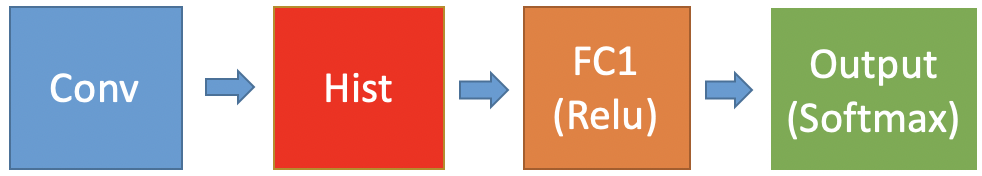
\includegraphics[width=\textwidth]{1CNN.png}
		\caption{1CNN}
	\end{subfigure}
	\hfill
	\begin{subfigure}[b]{.30\textwidth}
		\centering
		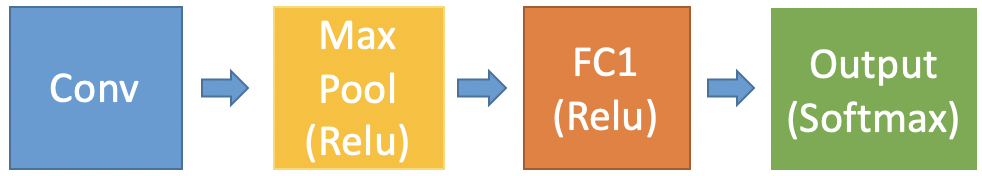
\includegraphics[width=\textwidth]{1HistCNN.png}
		\caption{1HistCNN}
	\end{subfigure}
	\hfill
	\begin{subfigure}[b]{.30\textwidth}
		\centering
		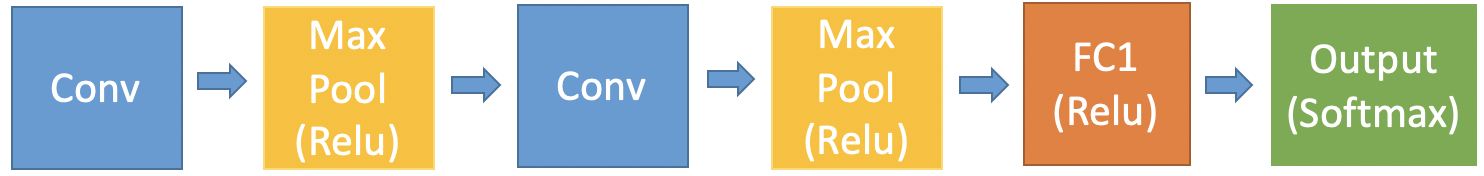
\includegraphics[width=\textwidth]{2CNN.png}
		\caption{2CNN}
	\end{subfigure}
	
	\begin{subfigure}[b]{.30\textwidth}
		\centering
		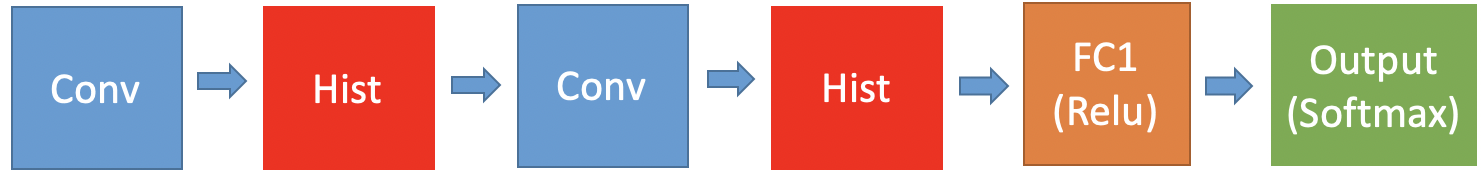
\includegraphics[width=\textwidth]{2HistCNN.png}\vspace{.55cm}
		\caption{2HistCNN}
	\end{subfigure}
	\hfil
	\begin{subfigure}[b]{.30\textwidth}
		\centering
		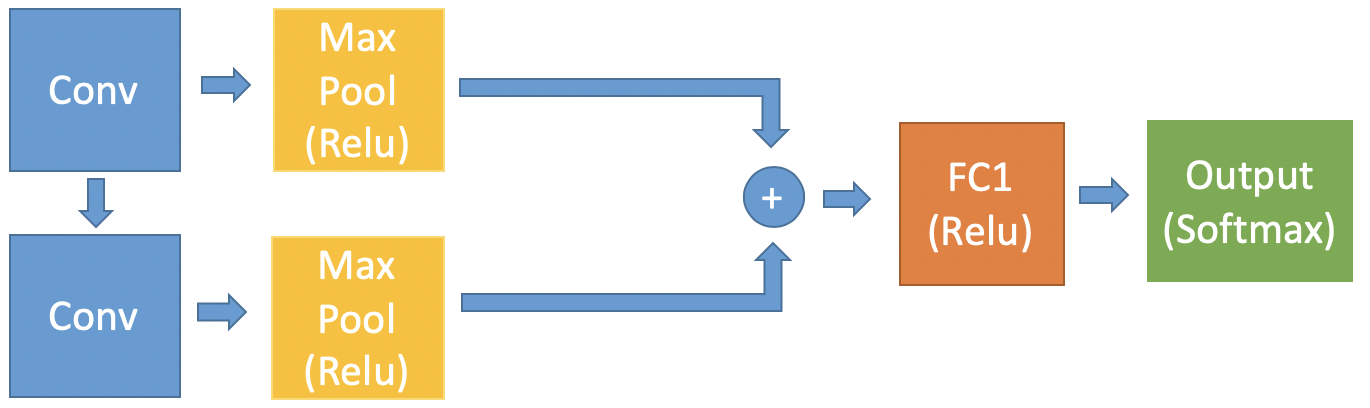
\includegraphics[width=\textwidth]{2CNN_parallel.png}
		\caption{2CNN Parallel}
	\end{subfigure}
	\hfil
	\begin{subfigure}[b]{.30\textwidth}
		\centering
		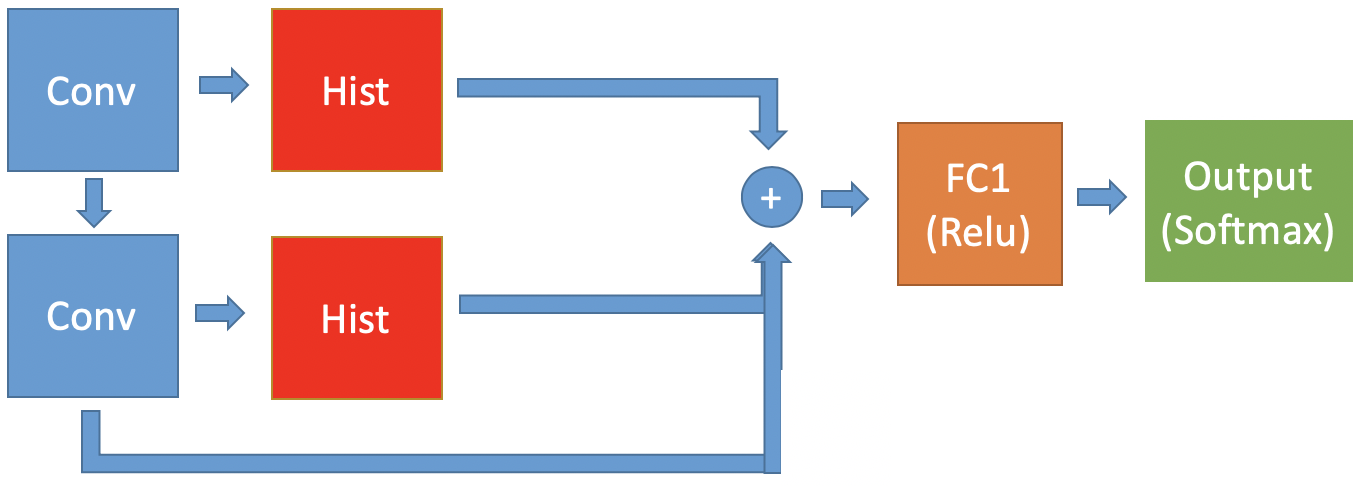
\includegraphics[width=\textwidth]{2HistCNN_parallel.png}
		\caption{2HistCNN Parallel}
	\end{subfigure}
	\caption{Architectures used for each texture dataset.}
	\label{fig:Networks}
\end{figure*}

\subsection{Binning Operation}

Binning operation in standard histogram can be expressed with the following counting fuction:
\begin{equation}
\label{eqn:cf}
y_k = \begin{cases}
1,B_k - w \leq x_k < B_k + w\\
0, otherwise
\end{cases}
\end{equation}

This indicator function returns 1 if the  element falls into a bin and returns 0 else. The condition when an element falls into a bin is defined by $B_k - w \leq x_k < B_k + w$, $B_k$ being the bin center and $w$ being the bin width. However, the standard histogram operation is not differentiable and cannot be used for the backpropagation \cite{Basu2018deeptexture}\cite{Wang2018learnable}.\\

Therefore, our approach is to perform a localized binning operation with a sliding window. RBFs will be used instead of the standard histogram operation to approximate the count values:

\begin{equation}
\label{eqn:rbf}
y_k =
\cfrac{1}{MN}\sum_{i=1}^{M}\sum_{j=1}^{N}e^{-\cfrac{\left(x_{ij}-\mu_k\right)^2}{\sigma_k^2}}.
\end{equation}

The function above returns the count $y_k$, for kth bin center $\mu_k$ and width $\sigma_k$ from the feature map value $x_{ij}$ . For RBFs, $\mu_k$ value controls the location of where the function is; therefore, this parameter has similar functionality to that of a bin center location for histogram. A similar comparison can be made with $w$ (bin width) and $\sigma_k$ it controls the scale (spread) of the distribution.

An example with M$\times$N window in an image is shown in Figure \ref{fig:2_1_1}. Each square represents a pixel with a single intensity value (feature map value) of 1, 2, or 3. Every pixel will contribute to every bin but not equally due to the RBF we are using. 


\begin{figure}[]
	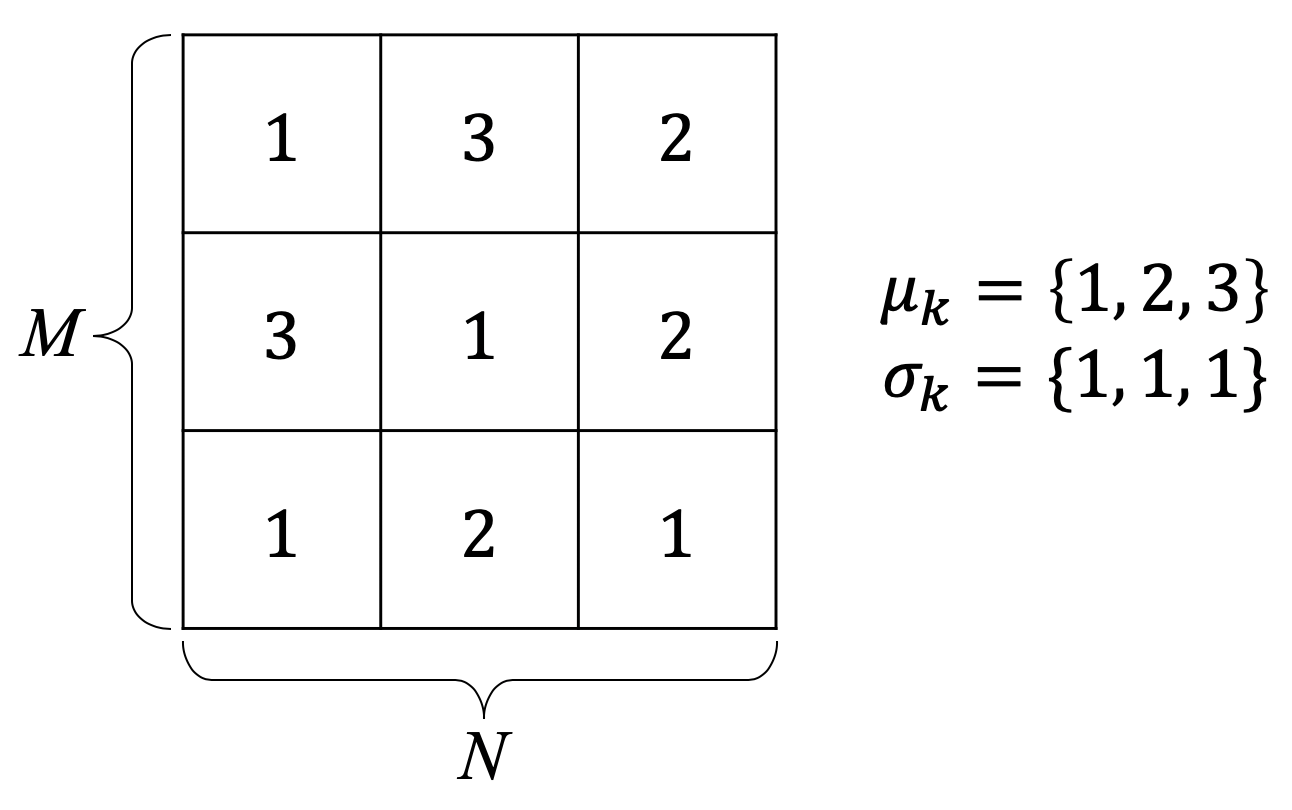
\includegraphics[width=1.0\linewidth]{2_1_1.png}
	\caption{M$\times$N Window}
	\label{fig:2_1_1}
\end{figure}

\begin{table}[t]
	\begin{tabular}{cccc}
		\hline
		\textbf{} & \textbf{\begin{tabular}[c]{@{}c@{}}$b_0$\\ Value: 1\end{tabular}} & \textbf{\begin{tabular}[c]{@{}c@{}}$b_1$\\ Value: 2\end{tabular}} & \textbf{\begin{tabular}[c]{@{}c@{}}$b_2$\\ Value: 3\end{tabular}} \\ \hline
		Standard & 0.44 & 0.33 & 0.22 \\ \hline
		RBF & 0.57 & 0.42 & 0.35 \\ \hline
	\end{tabular}
	\caption{Normalized Frequency Comparison}
	\label{tab:nfc}
\end{table}

Table \ref{tab:nfc} compares the resulting count value from the two equations introduced. Each column represents the bins, $b_0$, $b_1$ and $b_2$ each indicating bin center of 1, 2, and 3 respectively. The first row shows the value calculated by Equation \ref{eqn:cf} with $w = 0$, and the second row is based on Equation \ref{eqn:rbf}. RBF is used to approximate the counting function because it allows differentiation thereby allowing the model to learn via backpropagation. As shown in Figure \ref{fig:2_1_1}, $\sigma_k$ is set to be 1, which makes the difference between the two values larger. $\sigma_k$ is a crucial factor that determines this difference. As $\sigma_k$ value becomes smaller, the model will only consider the values that are very close to the bin center. If model learns the optimum $\sigma_k$ value, we will be able to account for ambiguity in the data as opposed to crisp histograms. As $\sigma_k$ value becomes larger, every element will fall into the same bin.

\begin{table}[]
	\begin{tabular}{@{}ccl@{}}
		\toprule
		\textbf{1\_CNN} & \textbf{2\_CNN} & \textbf{2\_CNN\_parallel} \\ \midrule
		10923 & 16583 & \multicolumn{1}{c}{65315} \\ \midrule
		\multicolumn{1}{l}{\textbf{1\_HistCNN}} & \multicolumn{1}{l}{\textbf{2\_HistCNN}} & \textbf{2\_HistCNN\_parallel} \\ \midrule
		10931 & 16579 & \multicolumn{1}{c}{65435} \\ \bottomrule
	\end{tabular}
	\caption{Number of Total Parameters for Each Network}
	\label{tab:parameter}
\end{table}

\begin{table*}[h!]
	\begin{tabular}{@{}ccccccc@{}}
		\toprule
		& \textbf{\begin{tabular}[c]{@{}c@{}}1\_CNN\\ Avg. F1-score\end{tabular}} & \textbf{\begin{tabular}[c]{@{}c@{}}1\_HistCNN\\ Avg. F1-score\end{tabular}} & \textbf{\begin{tabular}[c]{@{}c@{}}1\_CNN\\ Avg. Precision\end{tabular}} & \textbf{\begin{tabular}[c]{@{}c@{}}1\_HistCNN\\ Avg. Precision\end{tabular}} & \textbf{\begin{tabular}[c]{@{}c@{}}1\_CNN\\ Avg. Recall\end{tabular}} & \textbf{\begin{tabular}[c]{@{}c@{}}1\_HistCNN\\ Avg. Recall\end{tabular}} \\ \midrule
		Sample A & 0.45 $\pm$ 0.24 & 0.31 $\pm$ 0.28& 0.47 $\pm$ 0.22 & 0.30 $\pm$ 0.27 & 0.48 $\pm$ 0.29& 0.36 $\pm$ 0.32\\
		Sample B & 0.43 $\pm$ 0.22& 0.35 $\pm$ 0.29& 0.43 $\pm$ 0.21& 0.33 $\pm$ 0.30& 0.47 $\pm$ 0.27& 0.40 $\pm$ 0.32\\
		Sample C & 0.44 $\pm$ 0.25& 0.28 $\pm$ 0.28& 0.43 $\pm$ 0.24& 0.29 $\pm$ 0.31& 0.49 $\pm$ 0.28& 0.33 $\pm$ 0.33\\
		Sample D & 0.40 $\pm$ 0.23& 0.35 $\pm$ 0.30& 0.42 $\pm$ 0.22& 0.35 $\pm$ 0.29& 0.46 $\pm$ 0.29& 0.41 $\pm$ 0.32\\ \bottomrule
	\end{tabular}
	\caption{1\_CNN \& 1\_HistCNN}
	\label{tab:1cnn}
	
\end{table*}

\begin{table*}[h!]
	\begin{tabular}{@{}ccccccc@{}}
		\toprule
		& \textbf{\begin{tabular}[c]{@{}c@{}}2\_CNN\\ Avg. F1-score\end{tabular}} & \textbf{\begin{tabular}[c]{@{}c@{}}2\_HistCNN\\ Avg. F1-score\end{tabular}} & \textbf{\begin{tabular}[c]{@{}c@{}}2\_CNN\\ Avg. Precision\end{tabular}} & \textbf{\begin{tabular}[c]{@{}c@{}}2\_HistCNN\\ Avg. Precision\end{tabular}} & \textbf{\begin{tabular}[c]{@{}c@{}}2\_CNN\\ Avg. Recall\end{tabular}} & \textbf{\begin{tabular}[c]{@{}c@{}}2\_HistCNN\\ Avg. Recall\end{tabular}} \\ \midrule
		Sample A & 0.40 $\pm$ 0.23 & 0.33 $\pm$ 0.25 & 0.41 $\pm$ 0.22& 0.31 $\pm$ 0.21& 0.44 $\pm$ 0.28& 0.41 $\pm$ 0.33\\
		Sample B & 0.40 $\pm$ 0.23& 0.37 $\pm$ 0.24 & 0.40 $\pm$ 0.21& 0.37 $\pm$ 0.24& 0.44 $\pm$ 0.26& 0.42 $\pm$ 0.31\\
		Sample C & 0.42 $\pm$ 0.22& 0.34 $\pm$ 0.25& 0.44 $\pm$ 0.22& 0.34 $\pm$ 0.22& 0.46 $\pm$ 0.29& 0.40 $\pm$ 0.34\\
		Sample D & 0.38 $\pm$ 0.24& 0.32 $\pm$ 0.24& 0.40 $\pm$ 0.24& 0.31 $\pm$ 0.22& 0.43 $\pm$ 0.27& 0.38 $\pm$ 0.32\\ 	\bottomrule
	\end{tabular}
	\caption{2\_CNN \& 2\_HistCNN}
	\label{tab:2cnn}
\end{table*}


\begin{table*}[h!]
	\begin{tabular}{@{}ccccccc@{}}
		\toprule
		& \textbf{\begin{tabular}[c]{@{}c@{}}2\_CNN\_par\\ Avg. F1-score\end{tabular}} & \textbf{\begin{tabular}[c]{@{}c@{}}2\_HistCNN\_par\\ Avg. F1-score\end{tabular}} & \textbf{\begin{tabular}[c]{@{}c@{}}2\_CNN\_par\\ Avg. Precision\end{tabular}} & \textbf{\begin{tabular}[c]{@{}c@{}}2\_HistCNN\_par\\ Avg. Precision\end{tabular}} & \textbf{\begin{tabular}[c]{@{}c@{}}2\_CNN\_par\\ Avg. Recall\end{tabular}} & \textbf{\begin{tabular}[c]{@{}c@{}}2\_HistCNN\_par\\ Avg. Recall\end{tabular}} \\ \midrule
		Sample A & 0.44 $\pm$ 0.26& 0.31 $\pm$ 0.26& 0.45 $\pm$ 0.24& 0.31 $\pm$ 0.31& 0.48 $\pm$ 0.31& 0.36 $\pm$ 0.31\\
		Sample B & 0.44 $\pm$ 0.24& 0.31 $\pm$ 0.27 & 0.48 $\pm$ 0.23& 0.31 $\pm$ 0.30& 0.46 $\pm$ 0.30& 0.36 $\pm$ 0.30\\
		Sample C & 0.45 $\pm$ 0.24& 0.38 $\pm$ 0.25& 0.46 $\pm$ 0.24& 0.39 $\pm$ 0.30& 0.49 $\pm$ 0.32& 0.43 $\pm$ 0.30\\
		Sample D & 0.42 $\pm$ 0.28& 0.31 $\pm$ 0.26& 0.43 $\pm$ 0.24& 0.35 $\pm$ 0.31& 0.48 $\pm$ 0.33& 0.38 $\pm$ 0.30\\ \bottomrule
	\end{tabular}
	\caption{2\_CNN\_parallel \& 2\_HistCNN\_parallel}
	\label{tab:2cnnparallel}
\end{table*}

\subsection{Experiment Design}

\begin{figure}[H]
	\includegraphics[width=1.0\linewidth]{2_2_1.png}
	\caption{Example of KTH-TIPS 2b Images \cite{Mallikarjuna2006kth} }
	\label{fig:2_2_1}
\end{figure}


To evaluate the performance of the proposed model, we used KTH-TIPS 2b, a texture database with 4752 images classified into 11 categories with four samples in each class (A, B, C, D). We use six different artificial neural networks (ANN) that are comprised of convolutional and histogram layers to classify the images. We will compare the results both quantitatively and qualitatively. In qualitative analysis, confusion matrices are used to show the number of images that are classified correctly or incorrectly by each network. In quantitative analysis, we record the average accuracy, precision, recall, and F1 score.




Table \ref{tab:parameter} shows the number of parameters for each network. There are three pairs of networks each being comprised of 1 layer, 2 layers, and 2 parallel layers. Within each pair, we constrained the number of parameters to be as close as possible to evaluate the histogram CNN and standard CNN under similar architectures.

\subsection{Training Procedure}
For our training procedure, our data is first scaled to between 0 and 1. Next, we wanted to look at the effects of preprocessing our data through standardization

\begin{equation}
\label{eqn:std}
Z = \dfrac{x - \mu}{\sigma}.
\end{equation}

The Equation \ref{eqn:std} represents the standardization operation, where $x$ is the original feature value, $\mu$ is the mean of that feature value, $\sigma$  is its standard deviation, and $Z$ is the resulting standardized data. 
For our dataset, $x$ is the RGB value for each pixel and the corresponding mean ($\mu$) and standard deviation ($\sigma$) for each channel will be used to normalize the data through Equation \ref{eqn:std} . Data preprocessing is considered to be one of the most important components of training the model, and we want to compare the results from standardizing the data and relating this to the performance of each network. \\

For the training process, we use the same data augmentation and optimization technique for the six different neural networks shown in figure \ref{fig:Networks}. Similar to \cite{Xue2018dep}, all the samples were first resized to 128 $\times$ 128 then a crop of random size (0.8 to 1.0) of the original size and a random aspect ratio (3/4 to 4/3) of the original aspect ratio is extracted. This crop is finally resized to 112$\times$112 and horizontal flips ($p=0.5$) were used. The experiment starts with learning rate of 0.001 and batch size of 128. Throughout 100 total epochs, the learning rate decays by factor of 0.9 if model does not make significant changes within 10 epochs(threshold = 1e-4). During the learning rate decay, Adam, an adaptive learning rate optimization algorithm, is used. Adam allows for efficient stochastic optimization that only requires first-order gradients, allowing for little memory requirement\cite{kingma2014adam}. We trained on one sample and then tested on the other three.


\section{Result}

After all the scripts were executed in HiPerGator, University of Florida's cluster research supercomputer \cite{hp}, data were collected and analyzed with our own python scripts. Shown in Figure \ref{tab:accuracy}, average overall accuracy was computed for each network both for the networks that used standardized data and non-standardized data. The networks that used pre-processed data averaged 6.50\% better than networks that did not involve data-standardization in performance.
As it was shown that networks trained with standardized data had better performance, the rest of the analysis was only focused on results from these experiments. Additionally, the average F1-score, precision, and recall value was calculated to evaluate each network's performance more deeply. Tables \ref{tab:1cnn} through \ref{tab:2cnnparallel} each shows these collected values and compares between each standard CNN and histogram layer CNN pair for each sample runs. The figures \ref{fig:cm1} through \ref{fig:cm2p} shows the average confusion matrices for each model. The confusion matrices for each model in each sample run is attached in the appendix marked as figure \ref{fig:ap_cm1} through \ref{fig:ap_cm2p} Overall, all the networks showed strong performance in classifying brown\_bread, corduroy, and cork classes, which is shown with darker color in the corresponding blocks from the figure. On the other hand, most of the networks struggled on classifying aluminum\_foil, cotton, and white\_bread.\\

Along with confusion matrices, the histograms learned by the CNNs with histogram layer(s) can be found in the appendix (figures \ref{fig:histogram_2histcnn} through \ref{fig:histogram}). The number of bins are set to four, each curve in each figure represent a single bin, and the graph itself represents the bin center and bin width learned by each network for each sample run.

\section{Discussion}

\subsection{Standardization}

As mentioned above, the models were trained with standardized data and with non-standardized data. Table \ref{tab:accuracy} shows the average overall accuracy for six networks with columns divided into whether data was normalized or not. Normalization for data-processing is considered to be very important when training the model, and we were able to evaluate how the performance differs by the methods used for data-preprocessing.
As shown in Table \ref{tab:accuracy}, every network improved performance significantly with standardization, averaging about 6.50\% increase in average overall accuracy. From this result, we learned how normalizing the data before training can improve performance compared to using non-normalized dataset. In future works, standardization will continue to be used as a pre-processing technique for our data.


\subsection{Histogram Layer}

Based on Table \ref{tab:accuracy}, 2\_CNN\_parallel had the highest average overall accuracy followed by 1\_CNN. 2\_HistCNN showed the highest performance from the histogram CNNs.
Most of the histogram networks showed lower accuracy than the corresponding CNN except for 2HistCNN using unstandardized data.
However, since this is a multi-class problem, average overall accuracy alone cannot determine networks' performance. Therefore, we looked at average f1-score, precision, and recall shown in Table \ref{tab:1cnn} through \ref{tab:2cnnparallel} for further evaluation.\\

%%need more interpretation
From table \ref{tab:1cnn} through \ref{tab:2cnnparallel}, standard CNNs showed higher value both on average precision and recall than histogram CNNs, indicating that standard CNNs had lower false positives and more true positives. This ultimately led standard CNNs to have a higher average f1 score value.
Table \ref{tab:2cnn} compares 2\_CNN and 2\_HistCNN. 2\_CNN had mostly lower average f1-score, precision, and recall than 1\_CNN's, but 2\_HistCNN's f1-score, precision, and recall values were slightly higher than 1\_HistCNN. This is most likely because of an additional histogram layer.
For 2\_CNN\_parallel and 2\_HistCNN\_parallel shown in table \ref{tab:2cnnparallel}, f1-score, precision, and recall values were mostly similar with data from 1\_CNN and 1\_HistCNN.
%%

From these comparisons, we learned that the CNNs implemented with histogram layer did not necessarily perform better on texture classification. This may be due to insufficient tuning of parameters such as window size, kernel size, intialization method for histogram layer, and number of bins.


\subsection{Confusion Matrices} %I am not sure if this analysis is meaningful, but I wrote a draft based on what pattern I found.

Confusion matrices shown from figure \ref{fig:cm1} to \ref{fig:cm2p} reflects how different network performed in specific classes. The darkness of blue shade is proportional to model's performance in that class, and dark blue blocks should align diagonally (top left to bottom right) in an ideal situation. In general, the networks performed very well on brown\_bread, corduroy, and cork class but performed poorly on cotton, linen, and aluminum foil classes. By observing the distribution of the blue shades for other classes, there were focused false positive results for specific classes. Most of the networks, especially the non-histogram CNNs, predicted that the aluminum foil class was cork. On the other hand, classes such as cotton, cracker, lettuce leaf, and linen had more spread out false positive predictions unlike aluminum foil and wood classes. \\

Although most of the histogram CNNs did not necessarily perform better than the standard CNNs, they did show a better accuracy for some classes. For figure \ref{fig:cm1}, 1HistCNN performed better on cotton class. For figure \ref{fig:cm2}, 2HistCNN performed better on five classes (brown\_bread, corduroy, cork, wood, and linen). Lastly, for figure \ref{fig:cm2p}, 2HistCNN\_parallel performed better on three classes (Brown\_bread, corduroy, and cork). As these results suggest, histogram CNN showed stronger performance and confidence level on some classes.

\begin{figure}[t]
	\includegraphics[width=1.0\linewidth]{avg_cm1.png}
	\caption{Confusion Matrices for 1\_CNN (left) and 1\_HistCNN (right)}
	\label{fig:cm1}
\end{figure}

\begin{figure}[t]
	\includegraphics[width=1.0\linewidth]{avg_cm2.png}
	\caption{Average Confusion Matrices for 2\_CNN (left) and 2\_HistCNN (right)}
	\label{fig:cm2}
\end{figure}

\begin{figure}[t]
	\includegraphics[width=1.0\linewidth]{avg_cm3.png}
	\caption{Average Confusion Matrices for 2\_CNN\_parallel (left) and 2\_HistCNN\_parallel (right)}
	\label{fig:cm2p}
\end{figure}

The choice of which sample to use as testing set affected networks' performance in different classes as well. Although the blue shade distribution for cotton, cracker, lettuce leaf, and linen classes mostly looked random for A, B, and D test runs, networks trained with Sample C had more concentrated false positive predictions. Additionally, networks trained with Sample D had a similar effect on wood class. Unlike the other networks tested with A, B, and C sample, networks trained with Sample D showed strong confidence in predicting that the wood class texture images are wool. Sample D's data may have capured better information, such as illumination, pose, and scale, for that class.

From these analysis, we found that selection of which samples to use for training set affected the distribution of false positive results.

\begin{table}[t]
	\begin{tabular}{@{}ccc@{}}
		\toprule
		\multirow{2}{*}{Network} & \multicolumn{2}{c}{Average Overall Accuracy} \\ \cmidrule(l){2-3} 
		& Non-Standardized & Standardized \\ \midrule
		1\_CNN & 38.87 $\pm$ 4.05 & 47.48 $\pm$ 0.97 \\
		1\_HistCNN & 34.90 $\pm$ 4.09 & 37.43 $\pm$ 3.33 \\
		2\_CNN & 29.51 $\pm$ 5.14 & 44.35 $\pm$ 1.07 \\
		2\_HistCNN & 36.75 $\pm$ 2.58 & 40.14 $\pm$ 1.49 \\
		2\_CNN\_parallel & 40.31 $\pm$ 3.79 & 47.66 $\pm$ 1.22 \\
		2\_HistCNN\_parallel & 35.91 $\pm$ 4.15 & 38.20 $\pm$ 2.85 \\ \bottomrule
	\end{tabular}
	\caption{Average Overall Accuracy}
	\label{tab:accuracy}
\end{table}

\section{Conclusion}

In this paper, we have introduced a stackable histogram layer that involves localized binning operation on CNN. Based on analysis of overall accuracy, f1-score, precision, recall, and confusion matrix, histogram layer CNNs did not necessarily have better performance. However, some histogram layers performed better than CNNs on specific classes. This may be due to incomplete parameters tuning done prior to the experiments. There are still several different parameters that need to be considered such as the initialization method, number of bins, window size, and kernel size. For example, we used four bins, which may have not been enough for this experiment. Therefore, in future works, more parameters can be considered to determine if better performance will occur in these ANN architectures

\section{Acknowledgement}
I express my deepest and sincere gratitude to my mentor and UF graduate student Joshua Peeples who personally supervised, supported and encouraged me through the whole work. He supported me from learning basic concepts and math for machine learning to calculating torch size and tuning parameters. I would also like to thank him for proofreading this paper, allowing me to submit the best final version for presentation. He allowed me to get the most out of my summer research experience and greatly influenced my interest in computer science/machine learning field.

I would also like to thank University of Florida's Student Science Training Program (UF SSTP) and my lab host Dr. Alina Zare for making this research experience possible. Over the course of seven-weeks, I participated in this research in Dr. Alina Zare's Machine Learning and Sensing Lab. Working with other lab members and participating in weekly lab meetings helped me to understand the real university environment and this field more intuitively.

Lastly, I acknowledge University of Florida Research Computing for providing computational resources and support that have contributed to the research results reported in this publication.
URL: http://researchcomputing.ufl.edu



{\small
\bibliographystyle{ieee_fullname}
\bibliography{egbib}
}


\section{Appendix}

\begin{figure*}[htb]
	\centering
	\begin{subfigure}[b]{.20\textwidth}  % 1_HistCNN
		\centering
		\includegraphics[width=\textwidth]{1histcnn_a.eps}
		\caption{Sample A}
	\end{subfigure}
	\hfill
	\begin{subfigure}[b]{.20\textwidth}
		\centering
		\includegraphics[width=\textwidth]{1histcnn_b.eps}
		\caption{Sample B}
	\end{subfigure}
	\hfill
	\begin{subfigure}[b]{.20\textwidth}
		\centering
		\includegraphics[width=\textwidth]{1histcnn_c.eps}
		\caption{Sample C}
	\end{subfigure}
	\hfill
	\begin{subfigure}[b]{.20\textwidth}
		\centering
		\includegraphics[width=\textwidth]{1histcnn_d.eps}
		\caption{Sample D}
	\end{subfigure}
	
	\caption{Histograms learned for 1HistCNN}
	\label{fig:histogram_1cnn}
\end{figure*}

\begin{figure*}[htb]
	\centering	
	\begin{subfigure}[b]{.20\textwidth}  % 2_HistCNN_1
		\centering
		\includegraphics[width=\textwidth]{2histcnn_a_1.eps}
		\caption{Sample A}
		\label{subfig:2histcnn_1a}
	\end{subfigure}
	\hfill
	\begin{subfigure}[b]{.20\textwidth}
		\centering
		\includegraphics[width=\textwidth]{2histcnn_b_1.eps}
		\caption{Sample B}
	\end{subfigure}
	\hfill
	\begin{subfigure}[b]{.20\textwidth}
		\centering
		\includegraphics[width=\textwidth]{2histcnn_c_1.eps}
		\caption{Sample C}
	\end{subfigure}
	\hfill
	\begin{subfigure}[b]{.20\textwidth}
		\centering
		\includegraphics[width=\textwidth]{2histcnn_d_1.eps}
		\caption{Sample D}
		\label{subfig:2histcnn_1d}
	\end{subfigure}
	
	\begin{subfigure}[b]{.20\textwidth}  % 2_HistCNN_2
		\centering
		\includegraphics[width=\textwidth]{2histcnn_a_2.eps}
		\caption{Sample A}
		\label{subfig:2histcnn_2a}
	\end{subfigure}
	\hfill
	\begin{subfigure}[b]{.20\textwidth}
		\centering
		\includegraphics[width=\textwidth]{2histcnn_b_2.eps}
		\caption{Sample B}
	\end{subfigure}
	\hfill
	\begin{subfigure}[b]{.20\textwidth}
		\centering
		\includegraphics[width=\textwidth]{2histcnn_c_2.eps}
		\caption{Sample C}
	\end{subfigure}
	\hfill
	\begin{subfigure}[b]{.20\textwidth}
		\centering
		\includegraphics[width=\textwidth]{2histcnn_d_2.eps}
		\caption{Sample D}
		\label{subfig:2histcnn_2d}
	\end{subfigure}
	\caption{Histograms learned for 2\_HistCNN top row: 1st histogram layer (\ref{subfig:2histcnn_1a} - \ref{subfig:2histcnn_1d}); bottom row: 2nd histogram layer (\ref{subfig:2histcnn_2a} - \ref{subfig:2histcnn_2d})}
	\label{fig:histogram_2histcnn}
\end{figure*}

\begin{figure*}[htb]
	\centering	
	\begin{subfigure}[b]{.20\textwidth}  % 2_HistCNN_par_1
		\centering
		\includegraphics[width=\textwidth]{2histcnnpar_a_1.eps}
		\caption{Sample A}
		\label{subfig:2histcnnpar_1a}
	\end{subfigure}
	\hfill
	\begin{subfigure}[b]{.20\textwidth}
		\centering
		\includegraphics[width=\textwidth]{2histcnnpar_b_1.eps}
		\caption{Sample B}
	\end{subfigure}
	\hfill
	\begin{subfigure}[b]{.20\textwidth}
		\centering
		\includegraphics[width=\textwidth]{2histcnnpar_c_1.eps}
		\caption{Sample C}
	\end{subfigure}
	\hfill
	\begin{subfigure}[b]{.20\textwidth}
		\centering
		\includegraphics[width=\textwidth]{2histcnnpar_d_1.eps}
		\caption{Sample D}
		\label{subfig:2histcnnpar_1d}
	\end{subfigure}	
	
	\begin{subfigure}[b]{.20\textwidth}  % 2_HistCNN_par_2
		\centering
		\includegraphics[width=\textwidth]{2histcnnpar_a_2.eps}
		\caption{Sample A}
		\label{subfig:2histcnnpar_2a}
	\end{subfigure}
	\hfill
	\begin{subfigure}[b]{.20\textwidth}
		\centering
		\includegraphics[width=\textwidth]{2histcnnpar_b_2.eps}
		\caption{Sample B}
	\end{subfigure}
	\hfill
	\begin{subfigure}[b]{.20\textwidth}
		\centering
		\includegraphics[width=\textwidth]{2histcnnpar_c_2.eps}
		\caption{Sample C}
	\end{subfigure}
	\hfill
	\begin{subfigure}[b]{.20\textwidth}
		\centering
		\includegraphics[width=\textwidth]{2histcnnpar_d_2.eps}
		\caption{Sample D}
		\label{subfig:2histcnnpar_2d}
	\end{subfigure}
	\caption{Histograms learned for 2\_HistCNN\_parallel top row: 1st histogram layer (\ref{subfig:2histcnnpar_1a} - \ref{subfig:2histcnnpar_1d}); bottom row: 2nd histogram layer (\ref{subfig:2histcnnpar_2a} - \ref{subfig:2histcnnpar_2d})}
	\label{fig:histogram}
\end{figure*}

%%% Confusion Matrices
\begin{figure*}[]
	\includegraphics[width=0.7\linewidth]{appendix_cm1.png}
	\caption{Confusion Matrices for 1\_CNN (top row) and 1\_HistCNN (bottom row)}
	\label{fig:ap_cm1}
\end{figure*}

\begin{figure*}[]
	\includegraphics[width=0.7\linewidth]{appendix_cm2.png}
	\caption{Confusion Matrices for 2\_CNN (top row) and 2\_HistCNN (bottom row)}
	\label{fig:ap_cm2}
\end{figure*}

\begin{figure*}[]
	\includegraphics[width=0.7\linewidth]{appendix_cm3.png}
	\caption{Confusion Matrices for 2\_CNN\_parallel (top row) and 2\_HistCNN\_parallel (bottom row)}
	\label{fig:ap_cm2p}
\end{figure*}


\end{document}
